%%%%%%%%%%%%%%%%%%%% author.tex %%%%%%%%%%%%%%%%%%%%%%%%%%%%%%%%%%%
%
% sample root file for your "contribution" to a contributed volume
%
% Use this file as a template for your own input.
%
%%%%%%%%%%%%%%%% Springer %%%%%%%%%%%%%%%%%%%%%%%%%%%%%%%%%%%%%%%%%


%% RECOMMENDED %%%%%%%%%%%%%%%%%%%%%%%%%%%%%%%%%%%%%%%%%%%%%%%%%%%
%\documentclass[graybox]{svmult}
%
%% choose options for [] as required from the list
%% in the Reference Guide
%
%\usepackage{mathptmx}       % selects Times Roman as basic font
%\usepackage{helvet}         % selects Helvetica as sans-serif font
%\usepackage{courier}        % selects Courier as typewriter font
%\usepackage{type1cm}        % activate if the above 3 fonts are
                             % not available on your system
%
%\usepackage{makeidx}         % allows index generation
%\usepackage{graphicx}        % standard LaTeX graphics tool
%                             % when including figure files
%\usepackage{multicol}        % used for the two-column index
%\usepackage[bottom]{footmisc}% places footnotes at page bottom
%
%% see the list of further useful packages
%% in the Reference Guide
%
%\makeindex             % used for the subject index
%                       % please use the style svind.ist with
%                       % your makeindex program
%
%%%%%%%%%%%%%%%%%%%%%%%%%%%%%%%%%%%%%%%%%%%%%%%%%%%%%%%%%%%%%%%%%%%%%%%%%%%%%%%%%%%%%%%%%%
%
%\begin{document}

\title{Communities}
% Use \titlerunning{Short Title} for an abbreviated version of
% your contribution title if the original one is too long
\author{
    \textbf{Rodrigo Costa}
    \and{Ann-Margaret Esnard}
    \and{Henry Burton}}
\tocauthor{}
\authorrunning{Costa et al.}
% Use \authorrunning{Short Title} for an abbreviated version of
% your contribution title if the original one is too long
%\institute{Name of First Author \at Name, Address of Institute, %\email{name@email.address}
%\and Name of Second Author \at Name, Address of Institute %\email{name@email.address}}
%
% Use the package "url.sty" to avoid
% problems with special characters
% used in your e-mail or web address
%
\maketitle

A community can be defined as a place designated by geographical boundaries that functions under the jurisdiction of a governance structure, such as a town, city, or county \citep{kwasinski2016conceptual}. Communities are composed of physical, social, and economic infrastructure systems within these geographical boundaries, as well as the relationships between them. Our understanding of disaster recovery for individual systems has progressed significantly over the last decades. However, individual system analysis often lack recognition of dependencies on other systems, or do not holistically address the impacts to a community \citep{kwasinski2016conceptual}. Science-based measurement tools to evaluate recovery at community scales, integrated supporting databases, and risk-informed decision frameworks to support policies aimed at enhancing community resilience are at a rudimentary stage of development \citep{Ellingwood2016}. In short, modeling approaches for disaster recovery at the community level is still in its infancy. Yet, concepts of community recovery are valuable in developing recovery models with more limited scopes, e.g., for infrastructure, housing, or business recovery. This section introduces some of these key concepts that provide guidelines for the development of community recovery models. \ 

%--------------------------
\section{Concepts in Community Recovery Modeling} 
%--------------------------
Modeling community recovery requires a comprehensive understanding of post-disaster circumstances and conditions. This includes damage and serviceability of buildings and lifelines, their interactions with social and economic systems, the availability of human and financial resources for recovery activities, and the decisions made by relevant stakeholders \citep{deshmukh2012framework}. The challenges in modeling community start with the definition of what recovery looks like. Table \ref{tab:CommunityResilienceIndicators} provides a partial list of goals and indicators of community recovery. Different models may be required to evaluate the metrics in Table \ref{tab:CommunityResilienceIndicators}. Thus, the choice of the recovery metric will determine the most appropriate approach, data needs, and complexity of the community recovery model.\ 

%\begin{singlespace}
\begin{table}[tbh]
    \centering
   % \scriptsize
    \caption{Example of community recovery goals and indicators \citep{kwasinski2016conceptual,cutter2013disaster}.}
    \begin{tabularx}{\textwidth}{|l|X|}
    \toprule
    \textbf{Community performance goals} & \textbf{Examples of recovery indicators} \\ \midrule
    
    Population stability & Number of households dislocated; percent population remaining in the community; percent population remaining in homes; change in housing vacancy rate \\ \midrule
    
    Economic stability & Household income; employment; earnings by sector; assessed value of property; change in taxes and revenue (resources); change in gross city product (GCP) \\ \midrule
    
    Social services stability  & Hospital bed demand/supply ratio; school teacher/student ratio; availability of key retail and financial services \\ \midrule
    
    Physical services stability & Percent functionality of buildings and transportation systems; percent of population served by water, wastewater, electric power, gas, and telecommunication systems \\ \midrule
    
    Governance stability & Percent of population with access to police and fire protection and other essential public government services \\ 
    
    \bottomrule

    \end{tabularx}
    \label{tab:CommunityResilienceIndicators}
\end{table}
%\end{singlespace}

One of the early conceptual frameworks for the simulation of community disaster recovery was proposed by \cite{miles2003urban} and subsequently improved in \cite{Miles2006}. This conceptual framework is shown in Figure \ref{fig:CommunityRecovery}. It consists of three levels: lifelines, neighborhood, and community. Within these are the critical infrastructure networks, residential buildings and households, as well as business. The arrows in the figure indicates the interactions between these systems. Recent advances in the understanding of disaster recovery \citep{miles2019community} have demonstrated the complexity in these interactions. Nonetheless, this framework provides a solid foundation for the development of more sophisticated models for community disaster recovery. \ 

\begin{figure}[htb]
    \centering
    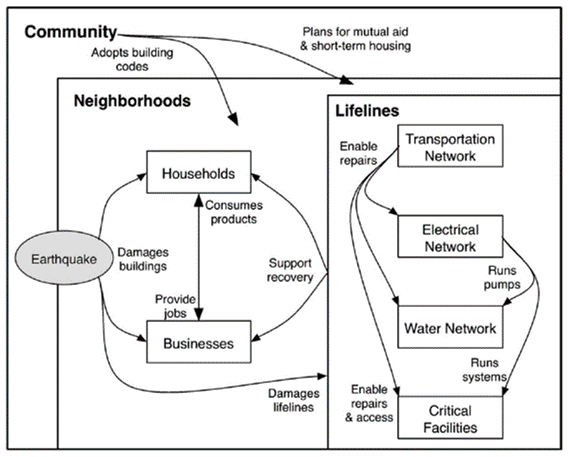
\includegraphics[width=0.8\textwidth, angle = 0]{Figures/CommunityRecovery.png}
    \caption{Conceptual model for community recovery \citep{miles2003urban}.}
    \label{fig:CommunityRecovery}
\end{figure}

To overcome some of the data constraints for community recovery modeling, the Centerville Virtual Community Testbed was developed as part of the NIST-funded Center of Excellence for Risk-based Community Resilience Planning initiative \citep{Ellingwood2016}. This testbed is aimed at enabling fundamental resilience assessment algorithms to be initiated, developed, and coded in a preliminary form, and tested before the refined measurement methods and supporting data classifications and databases necessary for a more complete assessment have fully matured. The Centerville testbed and other testbeds under development are a valuable resource for anyone developing models for community recovery.\ 

Simulation models for community recovery can greatly improve our ability to evaluate the benefits of selected mitigation measures. For example, the true benefits of retrofitting transportation infrastructure may be underestimated if the gains to the business sector are not accounted for. A more resilient business sector may also improve the recovery capacity of households. Thus, more than any model for the recovery of individual systems, fully integrated models for community recovery can greatly increase our capacity demonstrate the benefits of building resilience in our communities. 

\FloatBarrier
%--------------------------
\section{Major Research Gaps and Needs}
%--------------------------

A concerted and coordinated research effort is needed to do more and better modeling of community recovery. As per \citep{miles2019community}, part of this effort can simply be researching appropriate means of integrating existing infrastructure, housing, and business recovery models. The development of guidelines for the systematic collection of empirical data in future events is another area that requires more research. Empirical data play an important role in benchmarking and verification of simulation models, however, this type of data is still scarce. The development of virtual test-bed communities, for which detailed and granular information about infrastructure, buildings, households, and businesses is available can improve our ability to design community recovery models. Finally, collaborations between researchers from varied fields should be encouraged, facilitated, and rewarded. Community recovery is a multi-disciplinary subject, with physical, social, and economic dimensions. The creation of centers of excellence to foster multi-disciplinary approaches, facilitate information sharing, and develop partnerships with public and private sectors can greatly improve our understanding of this field.\ 

\FloatBarrier
%--------------------------
\section{Software and Systems}
%--------------------------
As discussed in the previous sections, the topic of recovery modeling has gained attention in recent years. Several modeling tools have been developed, as it will be demonstrated throughout this chapter. The innovations in these tools are briefly discussed in their respective sessions, and references are provided to those interested in obtaining more details. However, due to the large number of recovery modeling tools developed for specific-use, e.g., to study a specific problem and with limited transferability to other problems and contexts, these are not listed here. The following list only includes software and scripts that are targeted at simulating community recovery, and which are under continuous development with the intent of widespread use by the research community. These software and scripts include (or are in the process of including) models for infrastructure, businesses, buildings, as well as households, and are targeted at simulating systems of systems.\

\noindent\textbf{IN-CORE}\\ The Interdependent Networked Community Resilience Modeling Environment (IN-CORE) \citep{InCORE}. It was developed as a collaborative effort by researchers from different institutions and backgrounds, including social scientists, urban planners, and engineers. It contains modules for building and infrastructure loss assessments, economical, and sociological analysis. Although version 1.0 of IN-CORE has limited recovery modeling features, its strong multi-disciplinary foundation is expected to be leveraged for recovery assessments in future versions.\ 

\noindent\textbf{DESaster} \\is a Python library for discrete event simulation of disaster recovery. Currently, DESaster focuses on housing recovery. In the discrete-event framework of DESaster, the steps needed to repair residential buildings are the events, which include inspections, financing, and construction itself. An update for DESaster is expected in late 2020 to include critical infrastructure restoration and to integrate it to housing recovery modeling \citep{DESaster}.\ 

\noindent\textbf{RecovUS} \\ is a spatial agent-based model that includes spatial locations of homes and community assets and captures interactions of households with their neighbors and perceived community assets. It also simulates the effect of recovery of community, including infrastructure, neighbors, and community assets, on households’ recovery decisions \citep{moradi2020recovus}. 

\noindent\textbf{Rts} \\ is a framework of agent-based object-oriented models developed to study housing recovery \citep{costa2020housing}, and population displacements \citep{costa2020predicting}. The Rts framework includes models for water, power, and transportation infrastructure, resource suppliers, and buildings \citep{Costa2019thesis}. A sophisticated modeling approach for the simulation of the requests and the delivery of supplies is also implemented. \ 
